\documentclass[12pt,a4paper]{article} 

\usepackage{./fn2kursstyle}
\usepackage[russian]{babel}
\usepackage[T2A]{fontenc} 
\usepackage[utf8]{inputenc} 
\usepackage{geometry}
\usepackage{graphicx}
\usepackage{mathtools}
\usepackage{tikz}
\usepackage{pdfpages}
\usepackage{booktabs}
\usepackage{multirow,array}
\usepackage{siunitx}
\usepackage{amsmath}
\usepackage[hidelinks]{hyperref}

\counterwithout{equation}{section}
\counterwithout{figure}{section}
\graphicspath{{pic/}}
\frenchspacing 

\newcolumntype{C}[1]{>{\centering\arraybackslash}p{#1}}

\newcommand{\picref}[1]{рис. \ref{#1}}
\newcommand{\tabref}[1]{таблица \ref{#1}}
\newcommand{\half}{\frac{1}{2}}
\newcommand{\dhalf}{\dfrac{1}{2}}
\newcommand*{\Scale}[2][4]{\scalebox{#1}{$#2$}}

\title{Лабораторная работа №2 по дисциплине "Разработка программных комплексов" на тему "Численное решение дифференциального уравнения
	с граничными условиями проекционными методами"}
\group{ФН2-71Б}
\author{Пиневич В.\,Г.}
\supervisor{Азметов Х.\,Х.}
\date{2023}

\begin{document}
    \maketitle
    \tableofcontents
    \pagebreak

    \section{Задача}

    Создать программу решения дифференциального уравнения проекционными методами. Задано урванение на области $[0, 1]\colon$
    \[
        \dfrac{d^2 u}{dx^2} + u + x = 0.
    \]  

    Необходимо реализовать методы решения:
    \begin{enumerate}
        \item Метод Бубнова-Галеркина
        \item Метод Галеркина
        \item Метод наименьших квадратов
    \end{enumerate}
Реализовать методы учета граничных условий:
\begin{enumerate}
	\item Метод штрафа
	\item Метод множителей Лагранжа
\end{enumerate}

    По результатам предоставить отчет, в котором входят результаты для каждого метода
    решения с порядком аппроксимации 3, вариантами и методами учета граничных условий.
    Для метода штрафа задать значения 1, 100, 1000 и 10000..


    \pagebreak

    \section{ Метод Бубнова-Галеркина}
    
   	\subsection{Граничные условия $u(0) = 1; u(1) = 3$}

    \begin{center}
    	Метод штрафов
        \begin{tabular}{|c|c|c|c|} 
         \hline
         № & Штраф & Относительная ошибка & Коэффициенты приближенного решения \\ 
         \hline
         1 & 1 &$0.16$ & ${-4.37,6.47,-1.71}$ \\ 
         \hline
         2 & 10 &$0.02$ & ${-2.09,4.29,-1.24}$ \\ 
         \hline
         3 & 1000 &$0.01$ & ${-1.92,4.13,-1.21}$ \\ 
         \hline
         4 & 10000 &$0.01$ & ${-1.92,4.13,-1.21}$ \\ 
         \hline
        \end{tabular}
    \end{center}

    \begin{center}
	Метод множителей Лагранжа
	\begin{tabular}{|c|c|c|} 
		\hline
		№ & Относительная ошибка & Коэффициенты приближенного решения \\ 
		\hline
		1 & $0.01$ & ${-1.92,4.13,-1.21}$ \\ 
		\hline
	\end{tabular}
\end{center}

    \begin{figure}[h]
        \centering
        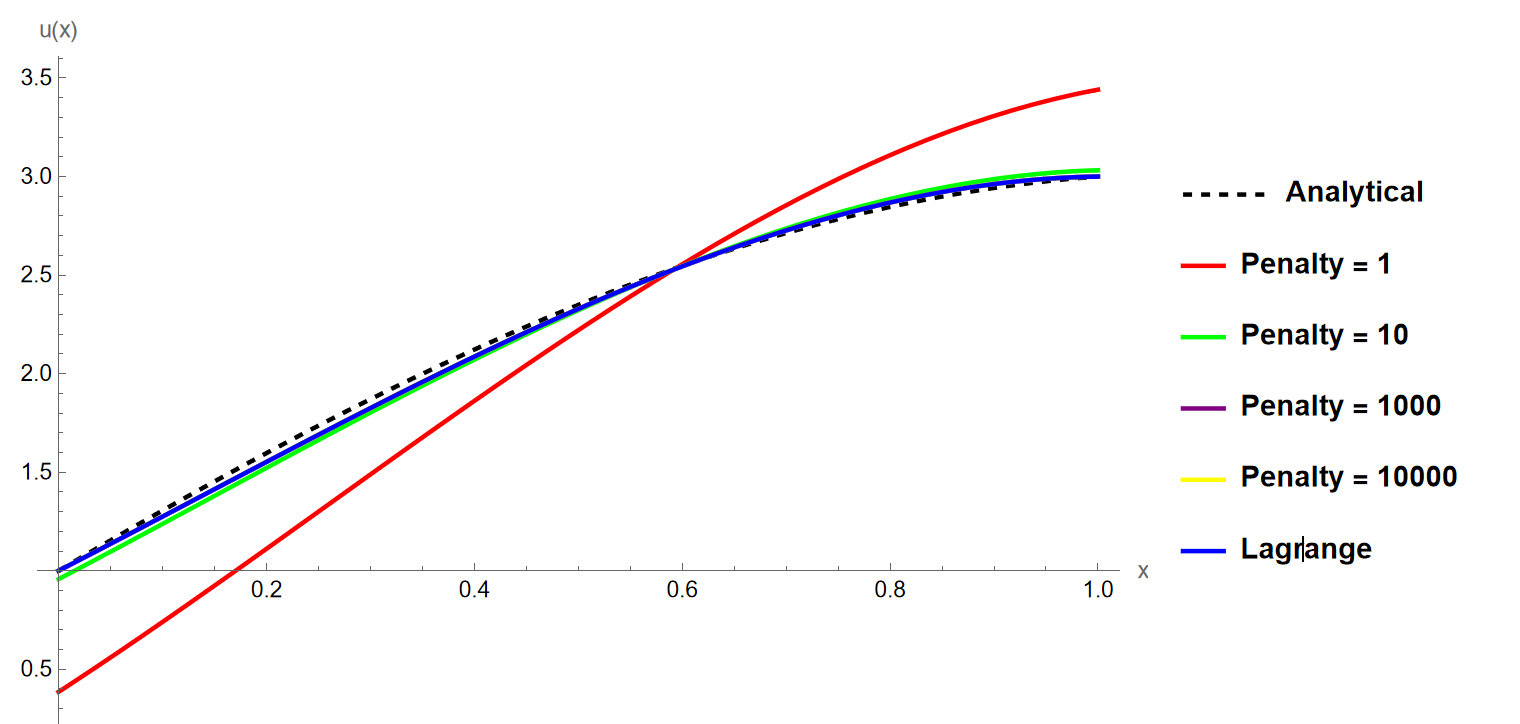
\includegraphics[width=1\textwidth]{m-1-1.PNG}
        \caption{График точного и численного решения метода Бубнова-Галеркина для $u(0) = 1; u(1) = 3$}
    \end{figure}

	\subsection{Граничные условия $u(0) = 1; u'(1) = 3$}
	
	    \begin{center}
		Метод штрафов
		\begin{tabular}{|c|c|c|c|} 
			\hline
			№ & Штраф & Относительная ошибка & Коэффициенты приближенного решения \\ 
			\hline
			1 & 1 &$0.40$ & ${-7.89,10.09,-2.44}$ \\ 
			\hline
			2 & 10 &$0.07$ & ${-7.36,11.02,-2.81}$ \\ 
			\hline
			3 & 1000 &$0.03$ & ${-7.29,11.14,-2.86}$ \\ 
			\hline
			4 & 10000 &$0.03$ & ${-7.28,11.14,-2.86}$ \\ 
			\hline
		\end{tabular}
	\end{center}
	
	\begin{center}
		Метод множителей Лагранжа
		\begin{tabular}{|c|c|c|} 
			\hline
			№ & Относительная ошибка & Коэффициенты приближенного решения \\ 
			\hline
			1 & $0.03$ & ${-7.28,11.14,-2.86}$ \\ 
			\hline
		\end{tabular}
	\end{center}
	
	\begin{figure}[h]
		\centering
		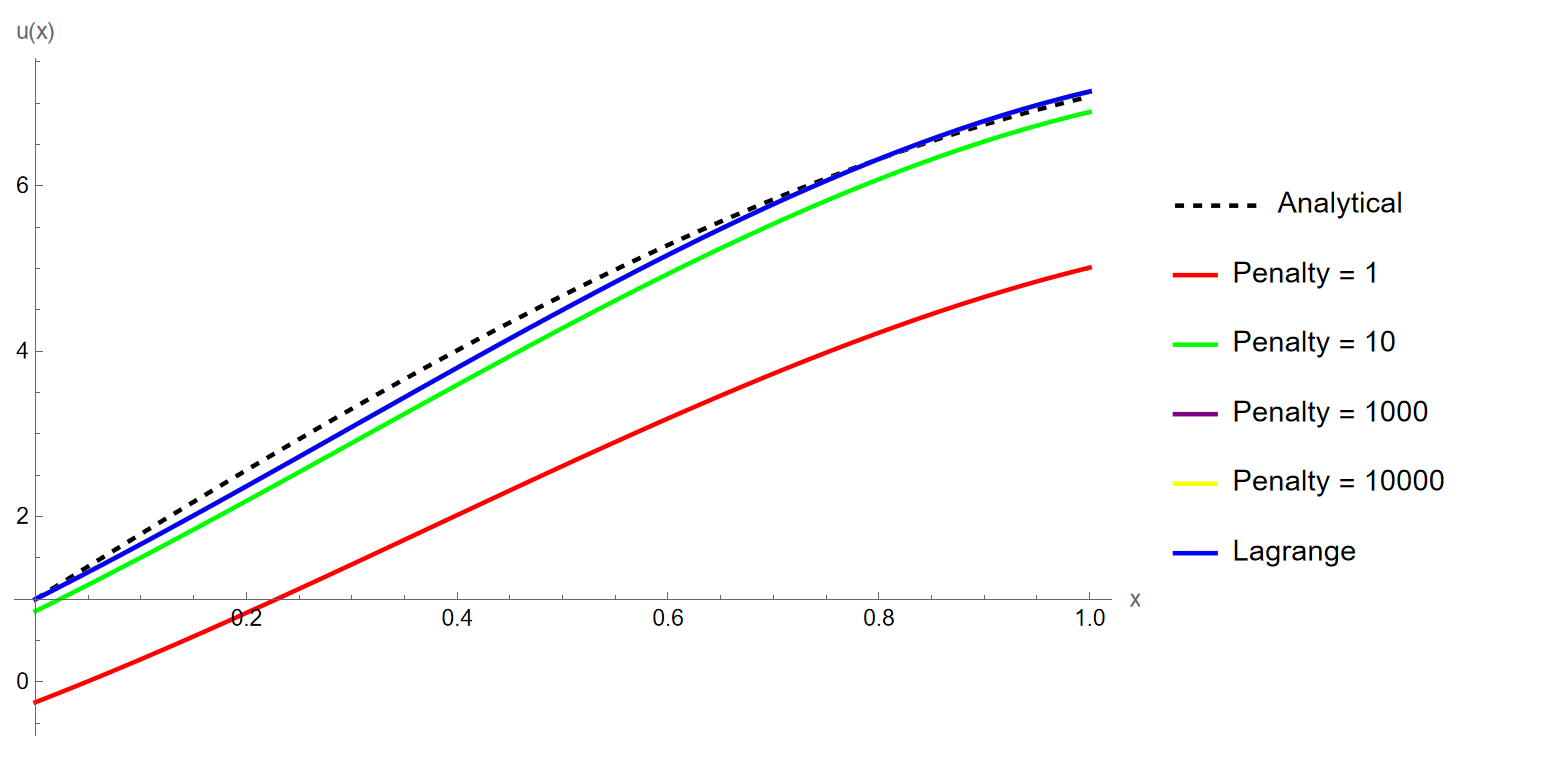
\includegraphics[width=1\textwidth]{m-1-2.PNG}
		\caption{График точного и численного решения метода Бубнова-Галеркина для $u(0) = 1; u'(1) = 3$}
	\end{figure}
	
	
	\subsection{Граничные условия $u'(0) = 1; u(1) = 3$}
	
	    \begin{center}
		Метод штрафов
		\begin{tabular}{|c|c|c|c|} 
			\hline
			№ & Штраф & Относительная ошибка & Коэффициенты приближенного решения \\ 
			\hline
			1 & 1 &$0.08$ & ${7.65,-4.10,0.48}$ \\ 
			\hline
			2 & 10 &$0.01$ & ${8.17,-4.34,0.50}$ \\ 
			\hline
			3 & 1000 &$0.00$ & ${8.23,-4.36,0.50}$ \\ 
			\hline
			4 & 10000 &$0.00$ & ${8.23,-4.36,0.50}$ \\ 
			\hline
		\end{tabular}
	\end{center}
	
	\begin{center}
		Метод множителей Лагранжа
		\begin{tabular}{|c|c|c|} 
			\hline
			№ & Относительная ошибка & Коэффициенты приближенного решения \\ 
			\hline
			1 & $0.00$ & ${8.23,-4.36,0.50}$ \\ 
			\hline
		\end{tabular}
	\end{center}
	
	\begin{figure}[h]
		\centering
		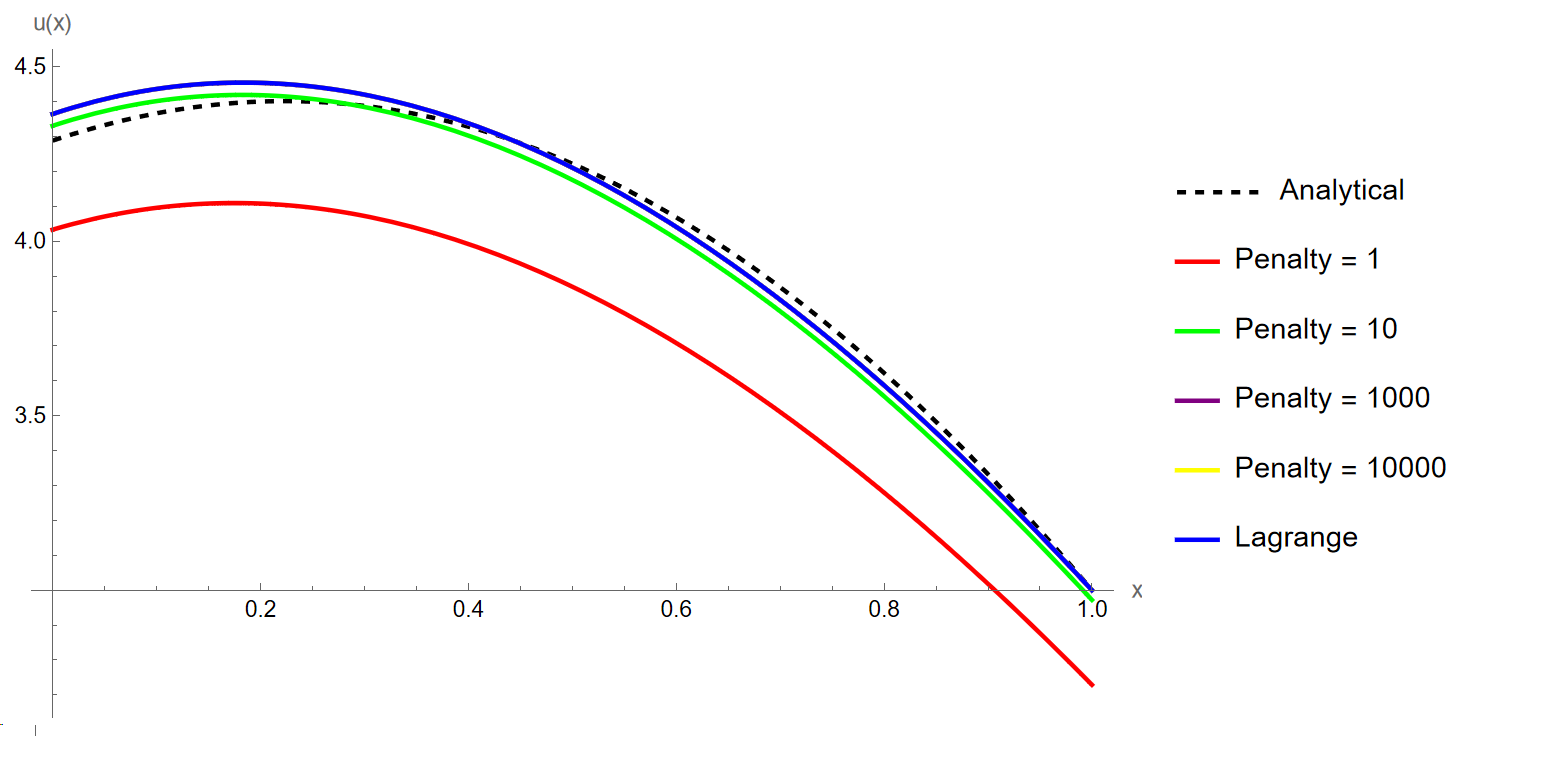
\includegraphics[width=1\textwidth]{m-1-3.PNG}
		\caption{График точного и численного решения метода Бубнова-Галеркина для $u'(0) = 1; u(1) = 3$}
	\end{figure}

    \pagebreak

    \section{ Метод Галеркина}

   	\subsection{Граничные условия $u(0) = 1; u(1) = 3$}

\begin{center}
	Метод штрафов
\begin{tabular}{|c|c|c|c|} 
	\hline
	№ & Штраф & Относительная ошибка & Коэффициенты приближенного решения \\ 
	\hline
	1 & 1 &$0.17$ & ${-0.37,3.07,-1.08}$ \\ 
	\hline
	2 & 10 &$0.04$ & ${-2.20,4.72,-1.44}$ \\ 
	\hline
	3 & 1000 &$0.03$ & ${-2.49,4.98,-1.49}$ \\ 
	\hline
	4 & 10000 &$0.03$ & ${-2.49,4.98,-1.49}$ \\ 
	\hline
\end{tabular}
\end{center}

\begin{center}
Метод множителей Лагранжа
\begin{tabular}{|c|c|c|} 
	\hline
	№ & Относительная ошибка & Коэффициенты приближенного решения \\ 
	\hline
	1 & $0.03$ & ${-2.49,4.98,-1.49}$ \\ 
	\hline
\end{tabular}
\end{center}

\begin{figure}[h]
	\centering
	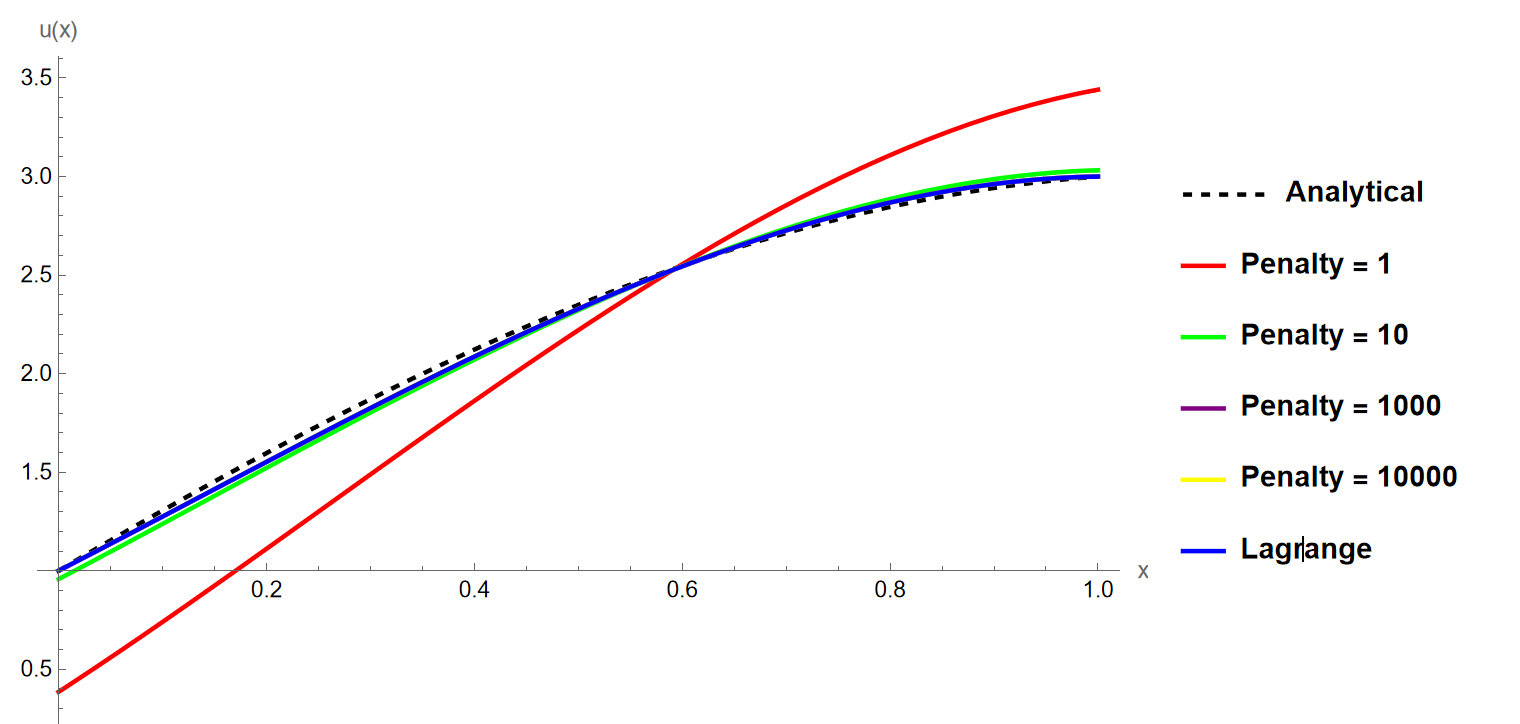
\includegraphics[width=1\textwidth]{m-2-1.PNG}
	\caption{График точного и численного решения метода Галеркина для $u(0) = 1; u(1) = 3$}
\end{figure}

\subsection{Граничные условия $u(0) = 1; u'(1) = 3$}

\begin{center}
	Метод штрафов
	\begin{tabular}{|c|c|c|c|} 
		\hline
		№ & Штраф & Относительная ошибка & Коэффициенты приближенного решения \\ 
		\hline
		1 & 1 &$8.39$ & ${-56.13,100.65,-28.72}$ \\ 
		\hline
		2 & 10 &$1.57$ & ${-27.17,39.29,-10.59}$ \\ 
		\hline
		3 & 1000 &$1.32$ & ${-26.09,37.00,-9.91}$ \\ 
		\hline
		4 & 10000 &$1.32$ & ${-26.08,36.98,-9.90}$ \\ 
		\hline
	\end{tabular}
\end{center}

\begin{center}
	Метод множителей Лагранжа
	\begin{tabular}{|c|c|c|} 
		\hline
		№ & Относительная ошибка & Коэффициенты приближенного решения \\ 
		\hline
		1 & $1.32$ & ${-26.08,36.98,-9.90}$ \\ 
		\hline
	\end{tabular}
\end{center}

\begin{figure}[h]
	\centering
	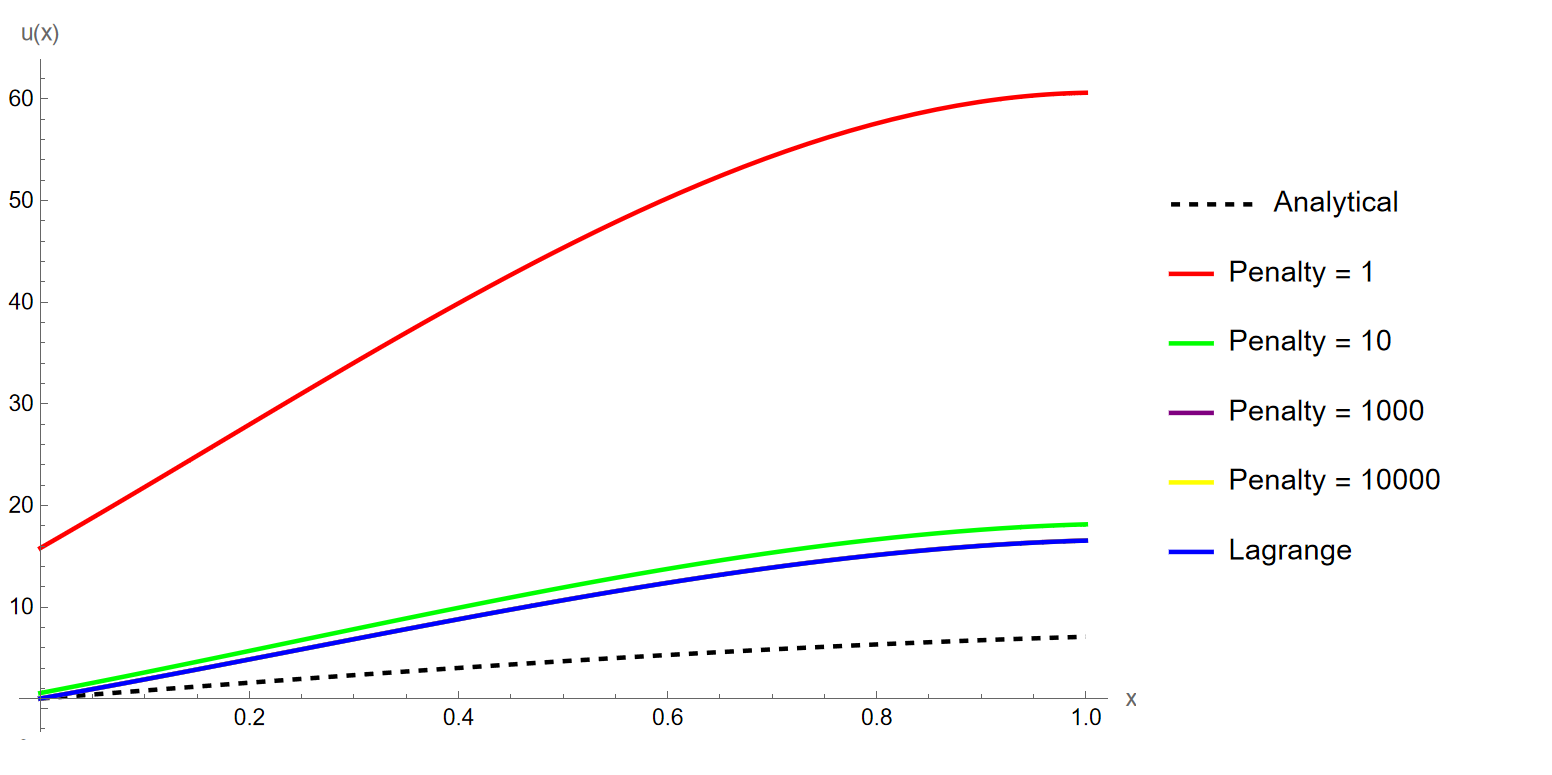
\includegraphics[width=1\textwidth]{m-2-2.PNG}
	\caption{График точного и численного решения метода Галеркина для $u(0) = 1; u'(1) = 3$}
\end{figure}

\subsection{Граничные условия $u'(0) = 1; u(1) = 3$}

\begin{center}
	Метод штрафов
	\begin{tabular}{|c|c|c|c|} 
		\hline
		№ & Штраф & Относительная ошибка & Коэффициенты приближенного решения \\ 
		\hline
		1 & 1 &$0.82$ & ${21.89,-15.21,2.59}$ \\ 
		\hline
		2 & 10 &$0.05$ & ${8.87,-4.79,0.55}$ \\ 
		\hline
		3 & 1000 &$0.03$ & ${8.54,-4.52,0.50}$ \\ 
		\hline
		4 & 10000 &$0.03$ & ${8.54,-4.52,0.50}$ \\ 
		\hline
	\end{tabular}
\end{center}

\begin{center}
	Метод множителей Лагранжа
	\begin{tabular}{|c|c|c|} 
		\hline
		№ & Относительная ошибка & Коэффициенты приближенного решения \\ 
		\hline
		1 & $0.03$ & ${8.54,-4.52,0.50}$ \\ 
		\hline
	\end{tabular}
\end{center}

\begin{figure}[h]
	\centering
	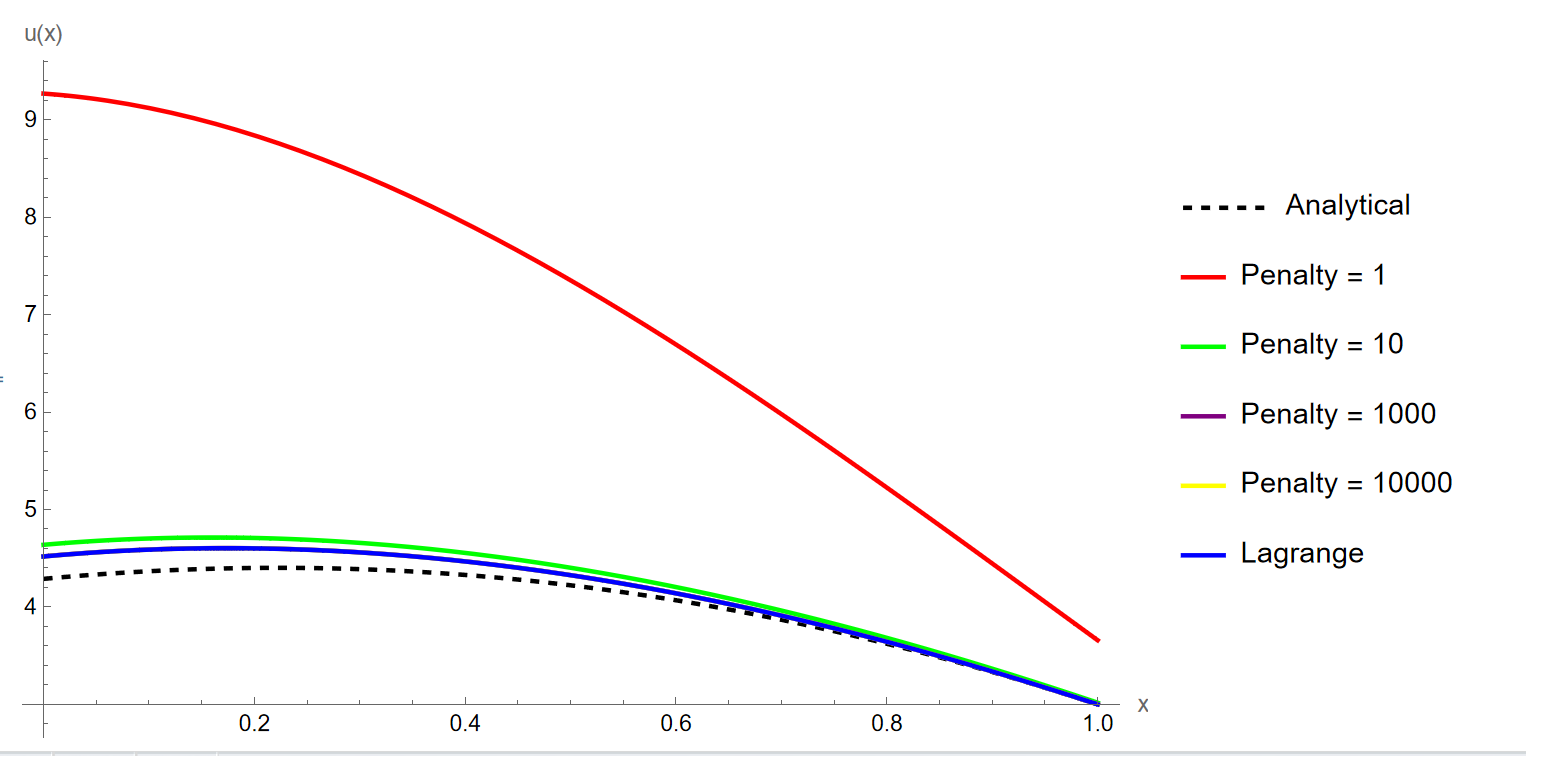
\includegraphics[width=1\textwidth]{m-2-3.PNG}
	\caption{График точного и численного решения метода Галеркина для $u'(0) = 1; u(1) = 3$}
\end{figure}


    \pagebreak

    \section{Метод наименьших квадратов}

   	\subsection{Граничные условия $u(0) = 1; u(1) = 3$}

\begin{center}
	Метод штрафов
	\begin{tabular}{|c|c|c|c|} 
		\hline
		№ & Штраф & Относительная ошибка & Коэффициенты приближенного решения \\ 
		\hline
		1 & 1 &$0.09$ & ${-0.16,2.25,-0.75}$ \\ 
		\hline
		2 & 10 &$0.03$ & ${-1.38,3.42,-1.0}$ \\ 
		\hline
		3 & 1000 &$0.03$ & ${-1.57,3.61,-1.04}$ \\ 
		\hline
		4 & 10000 &$0.03$ & ${-1.58,3.61,-1.04}$ \\ 
		\hline
	\end{tabular}
\end{center}

\begin{center}
	Метод множителей Лагранжа
	\begin{tabular}{|c|c|c|} 
		\hline
		№ & Относительная ошибка & Коэффициенты приближенного решения \\ 
		\hline
		1 & $0.03$ & ${-1.58,3.61,-1.04}$ \\ 
		\hline
	\end{tabular}
\end{center}

\begin{figure}[h]
	\centering
	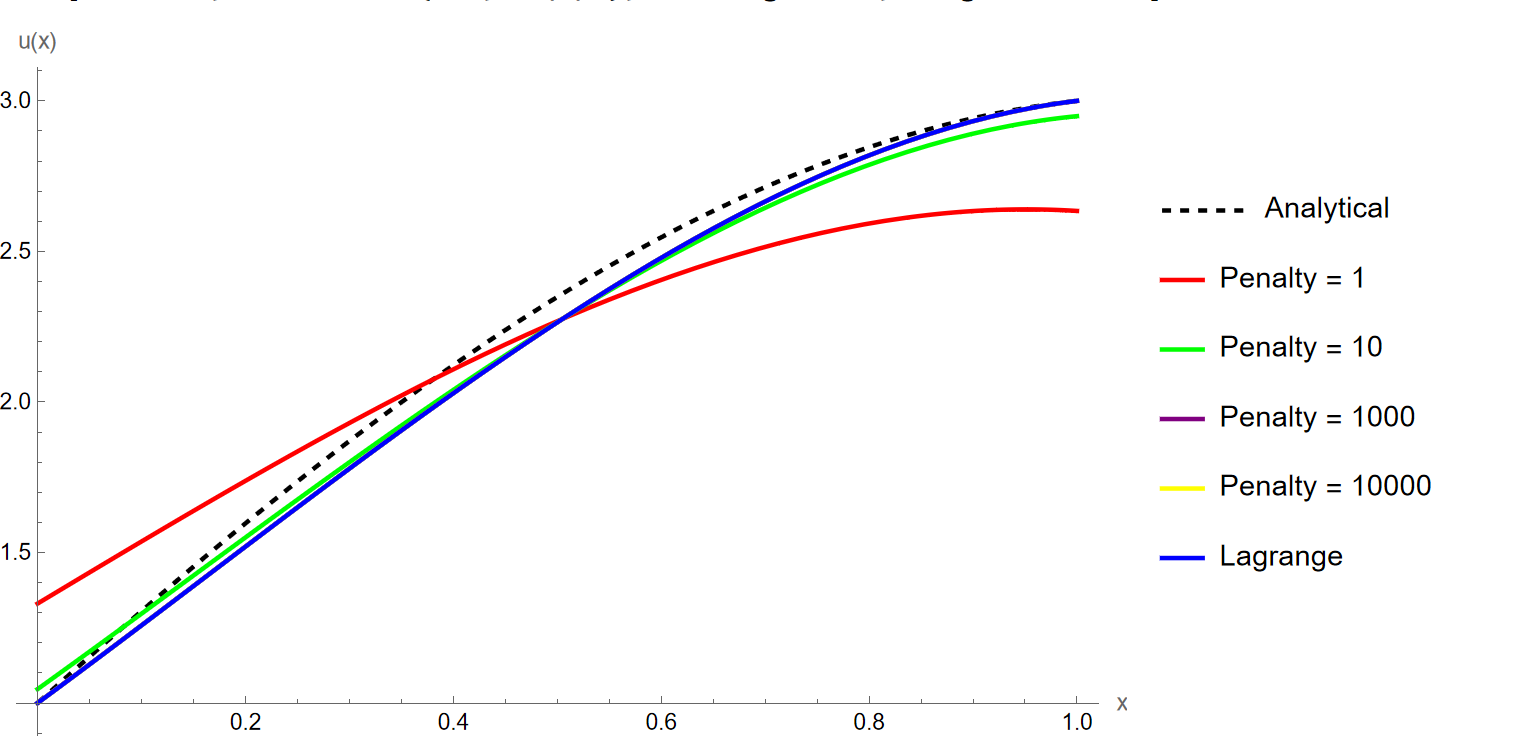
\includegraphics[width=1\textwidth]{m-3-1.PNG}
	\caption{График точного и численного решения метода наименьших квадратов для $u(0) = 1; u(1) = 3$}
\end{figure}

\subsection{Граничные условия $u(0) = 1; u'(1) = 3$}

\begin{center}
	Метод штрафов
	\begin{tabular}{|c|c|c|c|} 
		\hline
		№ & Штраф & Относительная ошибка & Коэффициенты приближенного решения \\ 
		\hline
		1 & 1 &$0.57$ & ${-3.41,4.92,-1.20}$ \\ 
		\hline
		2 & 10 &$0.26$ & ${-4.44,7.09,-1.76}$ \\ 
		\hline
		3 & 1000 &$0.20$ & ${-4.63,7.48,-1.86}$ \\ 
		\hline
		4 & 10000 &$0.20$ & ${-4.63,7.49,-1.86}$ \\ 
		\hline
	\end{tabular}
\end{center}

\begin{center}
	Метод множителей Лагранжа
	\begin{tabular}{|c|c|c|} 
		\hline
		№ & Относительная ошибка & Коэффициенты приближенного решения \\ 
		\hline
		1 & $0.20$ & ${-4.63,7.49,-1.86}$ \\ 
		\hline
	\end{tabular}
\end{center}

\begin{figure}[h]
	\centering
	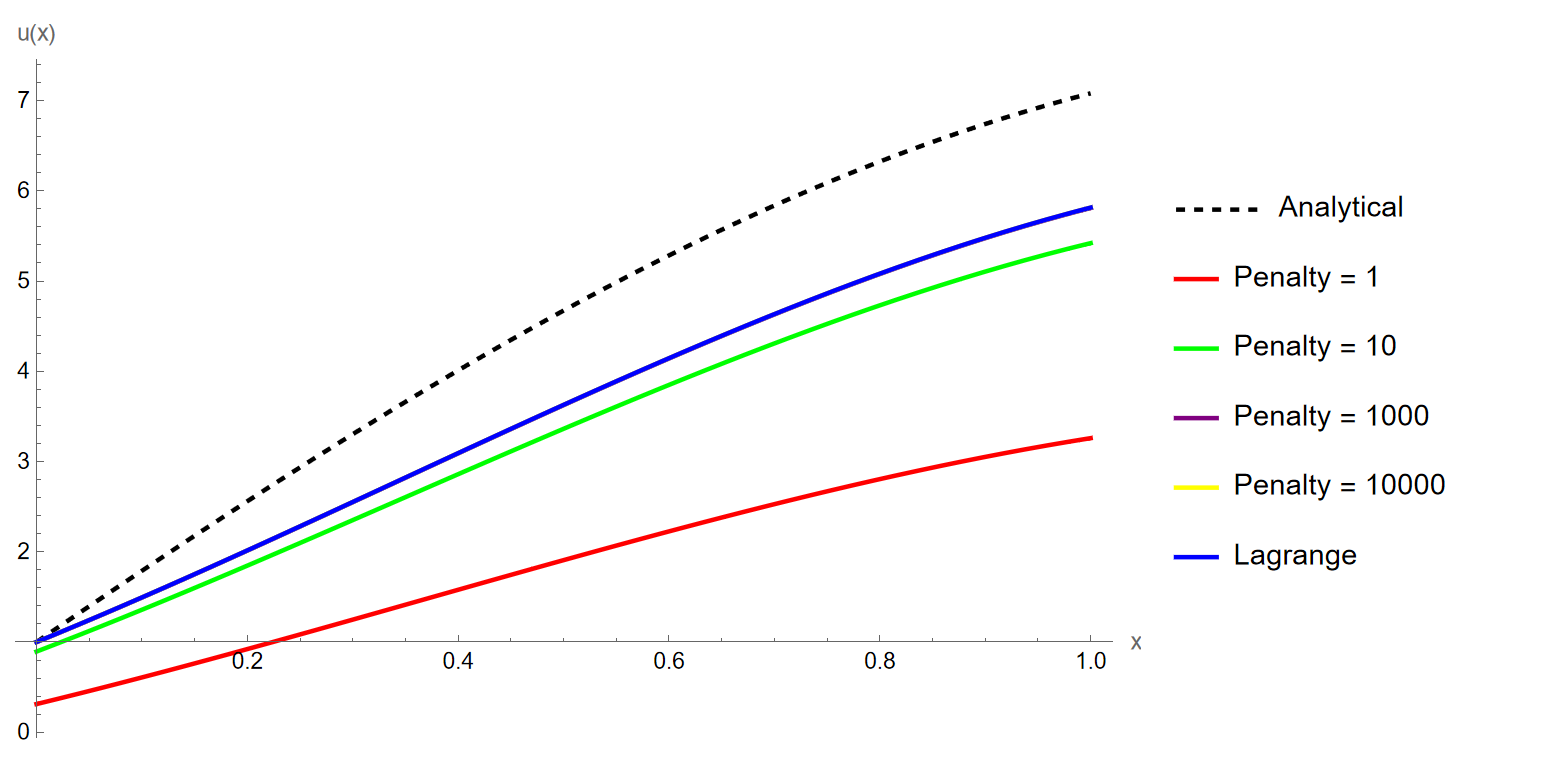
\includegraphics[width=1\textwidth]{m-3-2.PNG}
	\caption{График точного и численного решения метода наименьших квадратов для $u(0) = 1; u'(1) = 3$}
\end{figure}


\subsection{Граничные условия $u'(0) = 1; u(1) = 3$}

\begin{center}
	Метод штрафов
	\begin{tabular}{|c|c|c|c|} 
		\hline
		№ & Штраф & Относительная ошибка & Коэффициенты приближенного решения \\ 
		\hline
		1 & 1 &$0.10$ & ${6.24,-2.67,0.13}$ \\ 
		\hline
		2 & 10 &$0.06$ & ${8.32,-4.26,0.42}$ \\ 
		\hline
		3 & 1000 &$0.06$ & ${8.88,-4.69,0.50}$ \\ 
		\hline
		4 & 10000 &$0.06$ & ${8.88,-4.69,0.50}$ \\ 
		\hline
	\end{tabular}
\end{center}

\begin{center}
	Метод множителей Лагранжа
	\begin{tabular}{|c|c|c|} 
		\hline
		№ & Относительная ошибка & Коэффициенты приближенного решения \\ 
		\hline
		1 & $0.06$ & ${8.88,-4.69,0.50}$ \\ 
		\hline
	\end{tabular}
\end{center}

\begin{figure}[h]
	\centering
	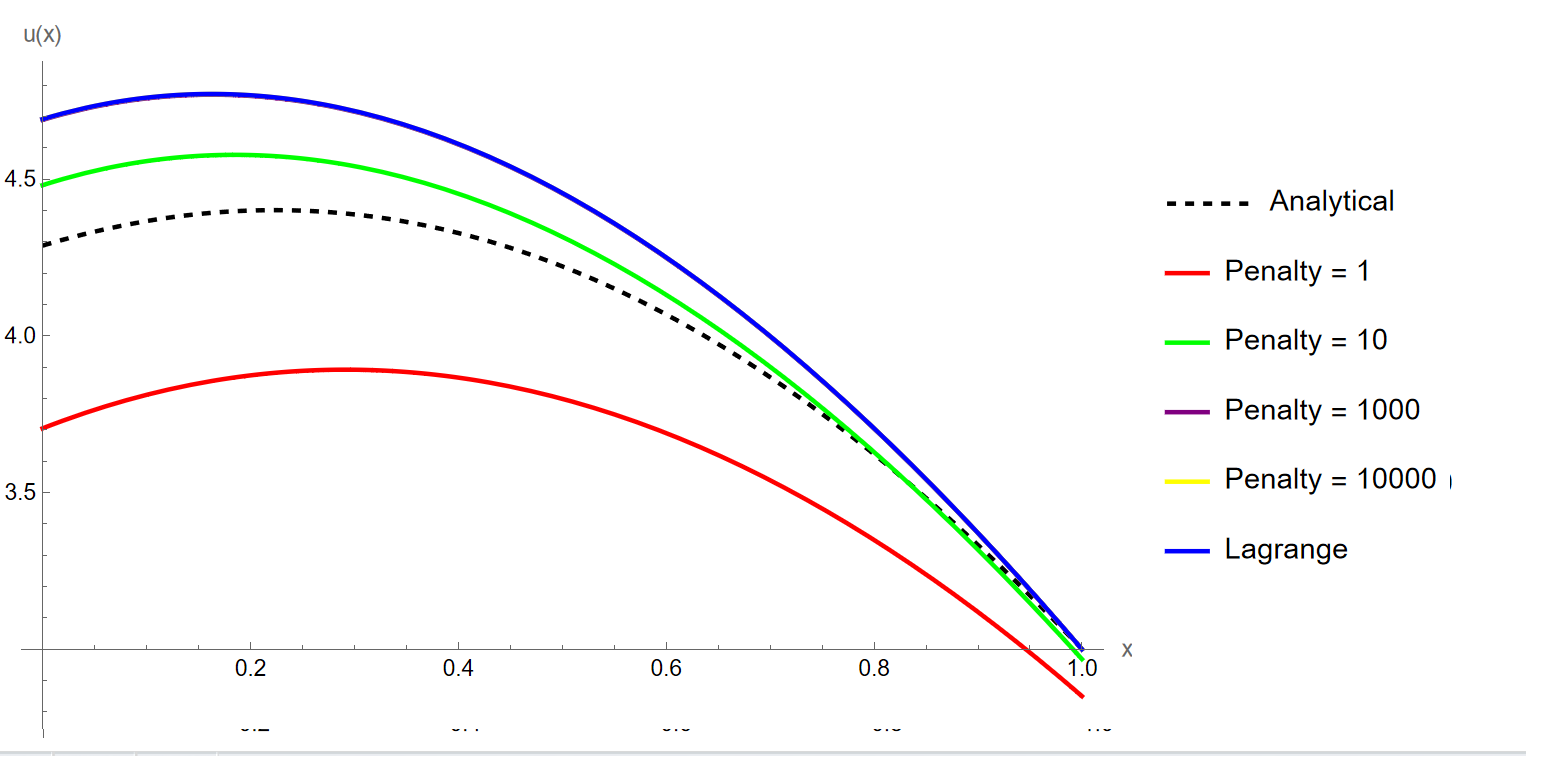
\includegraphics[width=1\textwidth]{m-3-3.PNG}
	\caption{График точного и численного решения метода наименьших квадратов для $u' (0) = 1; u(1) = 3$}
\end{figure}


    \pagebreak
\end{document}